% Compilar con python -m herramientas.informe; genera las secciones desde docs.
\documentclass[11pt,a4paper]{article}

\usepackage[spanish,es-noshorthands]{babel}
\usepackage{fontspec}
\usepackage[margin=2.4cm]{geometry}
\usepackage{microtype}
\usepackage{booktabs}
\usepackage{xltabular}
\usepackage{graphicx}
\usepackage{fancyvrb}
\usepackage{xcolor}
\usepackage{hyperref}
\usepackage{xurl}

% Fuentes incluidas en TeX Live; DejaVu cubre las flechas y símbolos que faltan.
\directlua{luaotfload.add_fallback("simbolos", {"file:DejaVuSerif.ttf:mode=harf;"})}
\setmainfont{LibertinusSerif}[Extension=.otf, UprightFont=*-Regular, BoldFont=*-Bold, ItalicFont=*-Italic, BoldItalicFont=*-BoldItalic, RawFeature={fallback=simbolos}]
\setmonofont{DejaVuSansMono}[Extension=.ttf, BoldFont=*-Bold, Scale=0.85]

\hypersetup{colorlinks, linkcolor=black, urlcolor=teal!70!black}
\fvset{fontsize=\small, frame=leftline, framerule=0.6pt, rulecolor=\color{gray!60}, xleftmargin=1em}
\setlength{\parindent}{0pt}
\setlength{\emergencystretch}{3em}
\setlength{\parskip}{0.6em}
\renewcommand{\arraystretch}{1.15}
\newcommand{\autoria}[1]{\emph{Autoría: #1.}\par}
\newcommand{\parte}[2]{\clearpage\phantomsection\addcontentsline{toc}{part}{#1}{\LARGE\bfseries #1\par}\vspace{0.3em}\autoria{#2}\vspace{0.6em}}

\newcommand{\repositorio}{https://github.com/Juanfra272/tc-proyecto1}

\begin{document}

\begin{titlepage}
  \centering
  \vspace*{3cm}
  {\large Teoría de la Computación (INFO1148)\par}
  \vspace{2cm}
  {\Huge\bfseries AgroReglas\par}
  \vspace{0.6cm}
  {\Large Diseño e implementación de un analizador sintáctico LL(1)\par}
  \vspace{2.5cm}
  {\large Fernando \quad Juanfra \quad Vicente\par}
  \vspace{1cm}
  {\url{\repositorio}\par}
  \vfill
  {\large Octubre de 2026\par}
\end{titlepage}

\tableofcontents

\parte{Definición y análisis formal}{Fernando}
\input{generado/teoria}

\parte{Diseño e implementación del parser}{Juanfra}
\input{generado/implementacion}

\parte{Integración, ejecución y casos de prueba}{Vicente}
\input{generado/integracion}

\clearpage
\phantomsection
\addcontentsline{toc}{part}{Conclusiones}
{\LARGE\bfseries Conclusiones\par}

AgroReglas cumple los mínimos del enunciado con siete palabras reservadas, seis operadores relacionales, dos conectores lógicos, varias reglas por programa y una extensión de negación y agrupación que forma parte de la gramática, la tabla, el parser y las pruebas.

La gramática final no tiene recursión izquierda ni prefijos comunes, y la tabla predictiva tiene 25 celdas ocupadas y ningún conflicto. Por eso el parser decide cada paso con un solo token de anticipación, sin retroceso. El verificador vuelve a calcular FIRST, FOLLOW y la tabla desde \texttt{especificacion/gramatica.json}, y el parser carga esa misma tabla, así que la teoría documentada y el código no pueden divergir sin que falle la verificación.

El parser usa una pila explícita en lugar de recursión, por lo que una entrada con 1100 paréntesis anidados se analiza sin alcanzar el límite de recursión de Python. Construye el AST en el mismo recorrido mediante reducciones y respeta la precedencia y la asociación izquierda acordadas.

Las 25 entradas documentadas obtienen el resultado esperado y cada rechazo informa la línea, la columna, el token encontrado y lo que se esperaba. La ejecución desde archivo o texto señala la posición del error en la línea original.

El parser solo comprueba sintaxis: no evalúa condiciones ni verifica que los sensores o dispositivos existan, y acepta comparaciones como \texttt{temperatura > TRUE}. Una etapa semántica posterior podría validar tipos y vocabulario del dominio sobre el AST que ya se construye.

\clearpage
\phantomsection
\addcontentsline{toc}{part}{Anexos}
{\LARGE\bfseries Anexos\par}

\section*{A. Código fuente}
\addcontentsline{toc}{section}{A. Código fuente}

El código fuente, la especificación, las pruebas, el README y este informe están en \url{\repositorio}. El README indica los requisitos, el formato de entrada y los comandos de ejecución.

\section*{B. Demostración funcional}
\addcontentsline{toc}{section}{B. Demostración funcional}

Las capturas muestran páginas generadas por \texttt{python -m herramientas.evidencia\_parser} con la salida real de Python.

\begin{figure}[h]
  \centering
  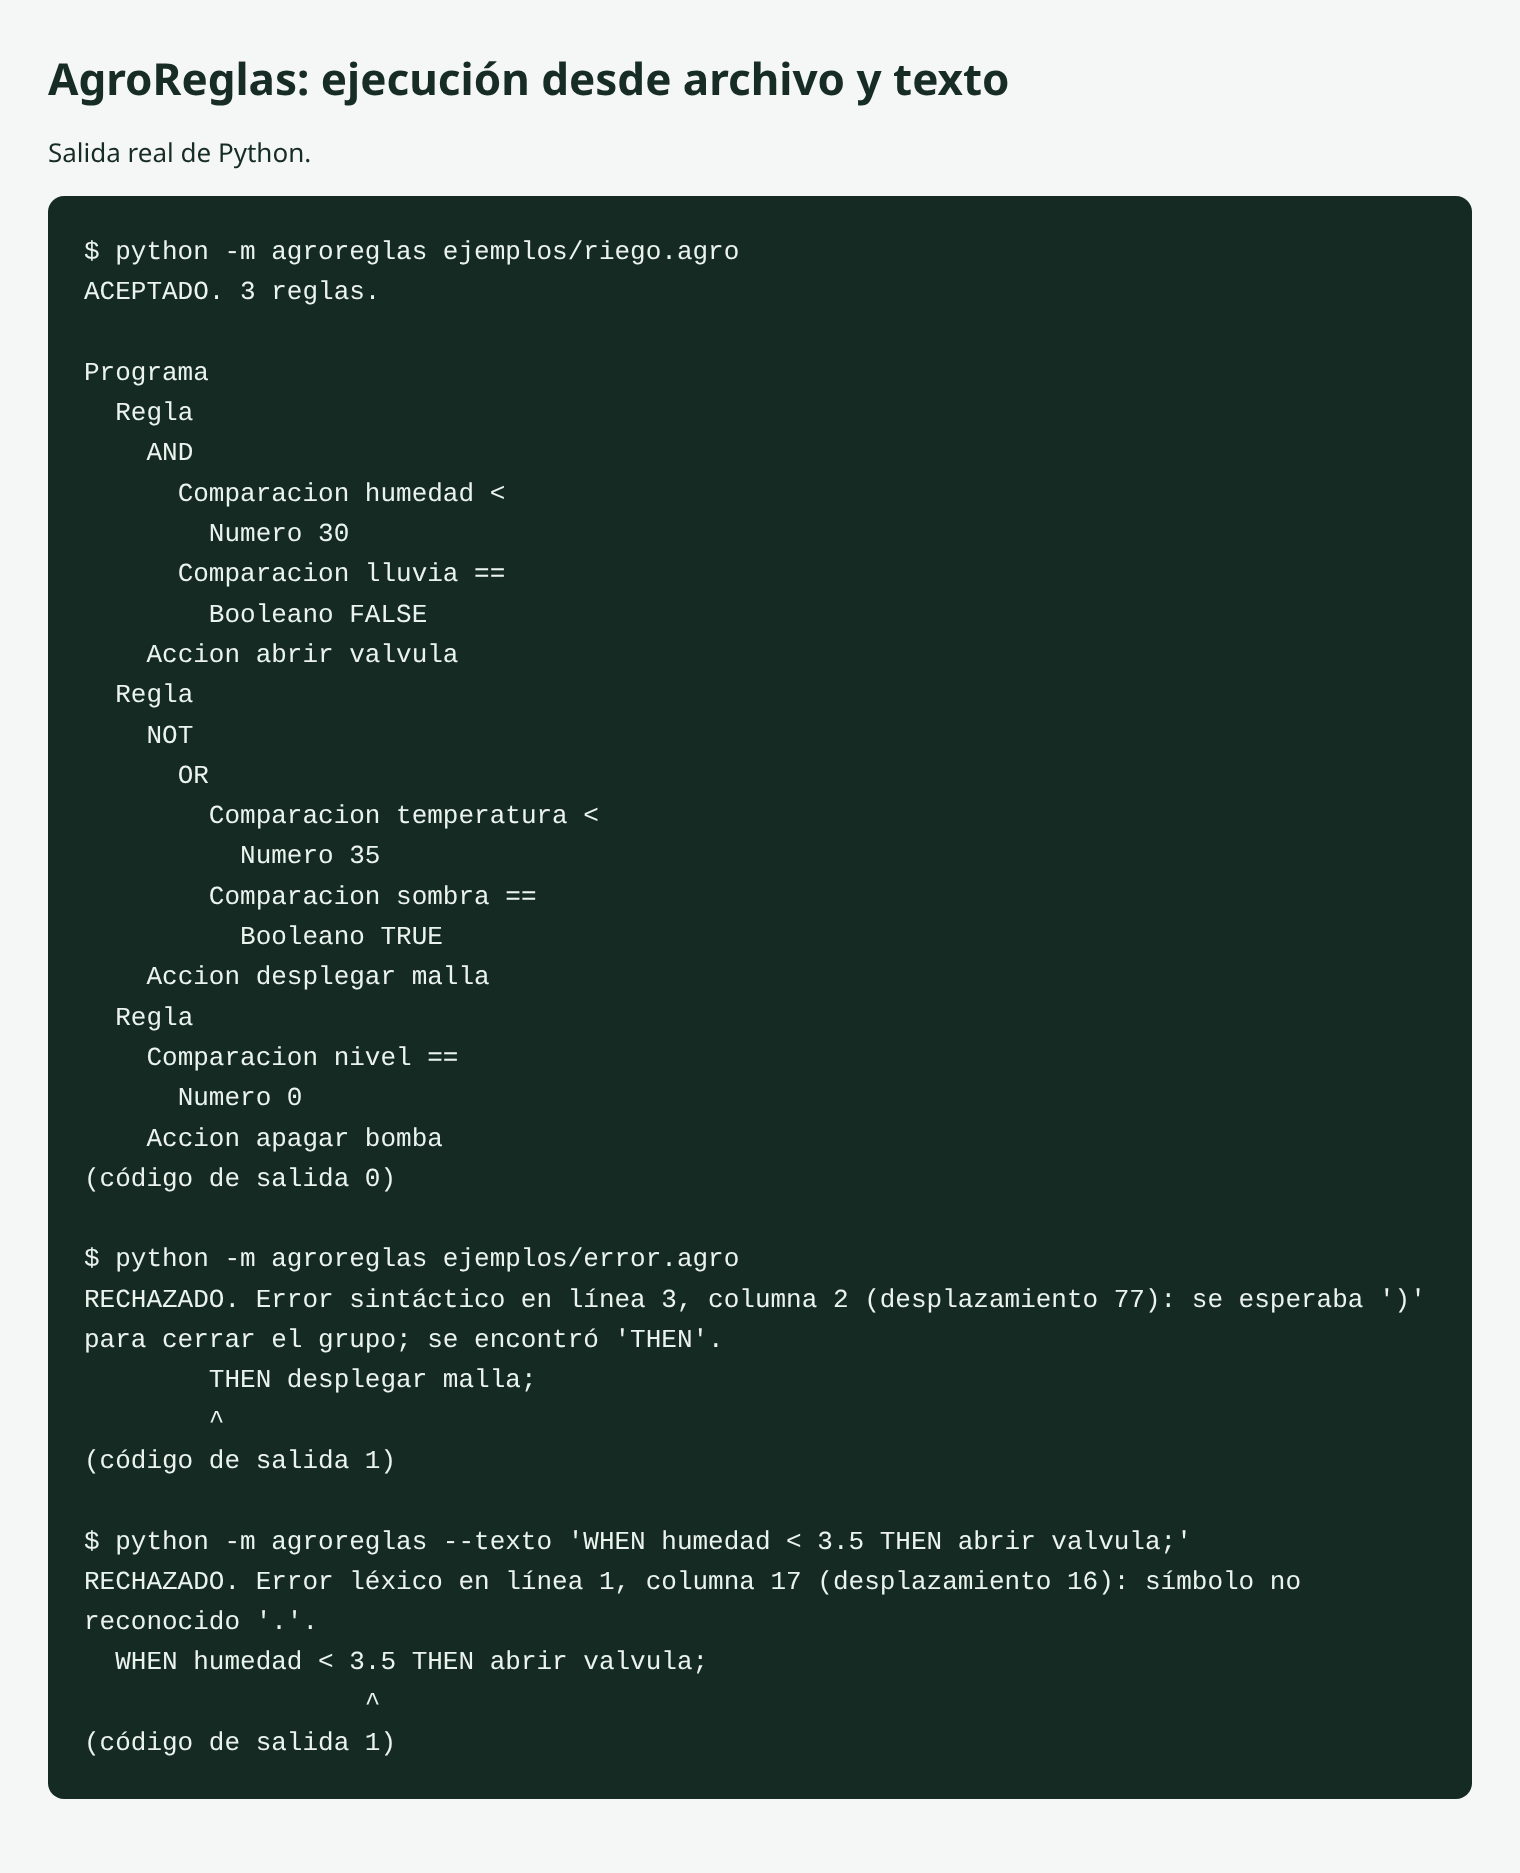
\includegraphics[width=\textwidth]{../docs/evidencias/cli.png}
  \caption{Ejecución desde archivo y desde texto: un programa aceptado con su AST, un error sintáctico en la tercera línea y un error léxico.}
\end{figure}

\begin{figure}[h]
  \centering
  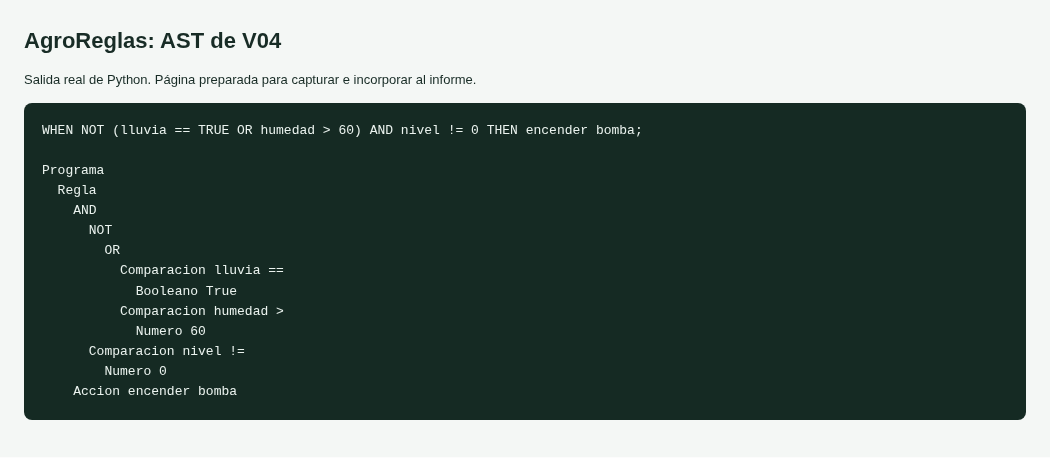
\includegraphics[width=\textwidth]{../docs/evidencias/arbol.png}
  \caption{AST del caso V04, con la negación sobre el grupo y el AND como raíz de la condición.}
\end{figure}

\begin{figure}[p]
  \centering
  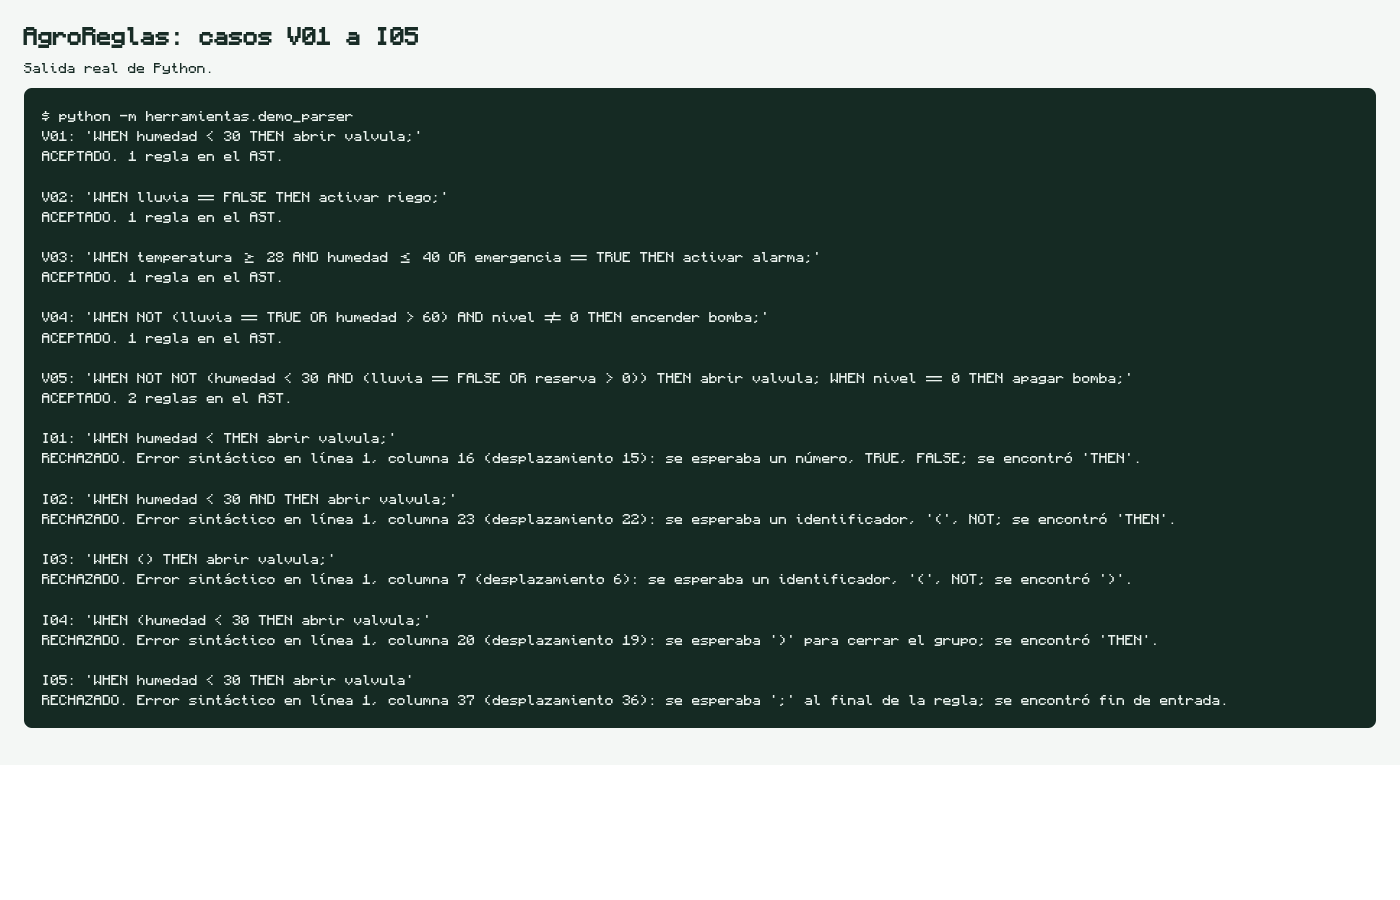
\includegraphics[width=\textwidth]{../docs/evidencias/ejecucion.png}
  \caption{Decisión del analizador en los diez casos de Fernando, con el mensaje completo de cada rechazo.}
\end{figure}

\begin{figure}[p]
  \centering
  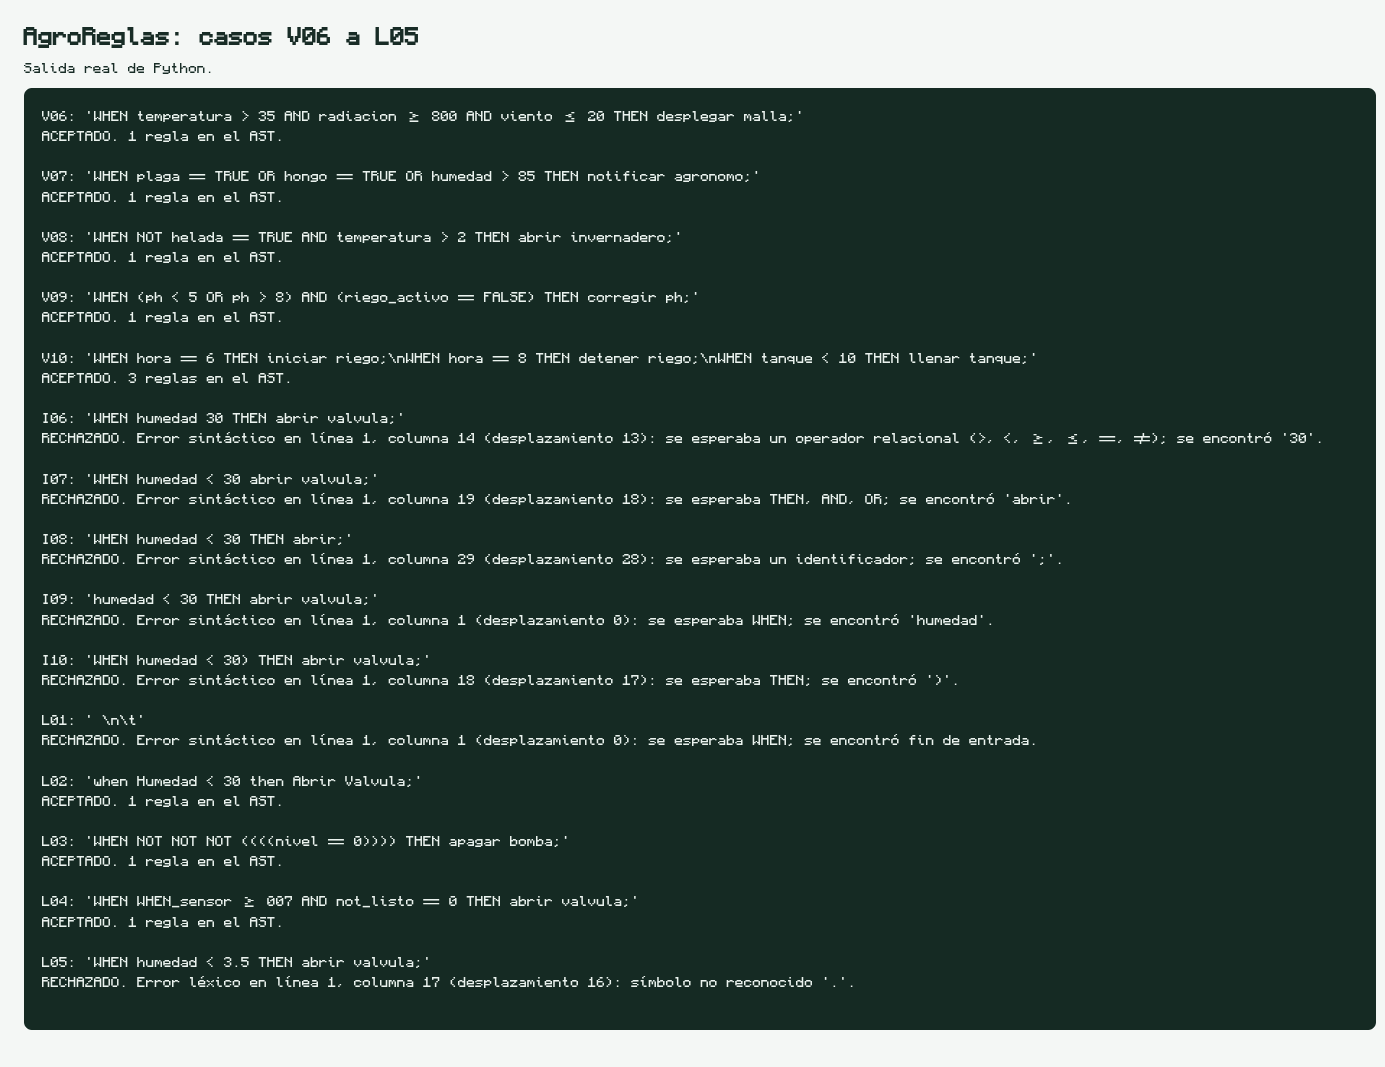
\includegraphics[width=\textwidth]{../docs/evidencias/ejecucion-nuevos.png}
  \caption{Decisión del analizador en los quince casos nuevos, incluidos los cinco casos límite.}
\end{figure}

\end{document}
